% Options for packages loaded elsewhere
\PassOptionsToPackage{unicode}{hyperref}
\PassOptionsToPackage{hyphens}{url}
%
\documentclass[
  ignorenonframetext,
  aspectratio=169,
]{beamer}
\usepackage{pgfpages}
\setbeamertemplate{caption}[numbered]
\setbeamertemplate{caption label separator}{: }
\setbeamercolor{caption name}{fg=normal text.fg}
\beamertemplatenavigationsymbolsempty
% Prevent slide breaks in the middle of a paragraph
\widowpenalties 1 10000
\raggedbottom
\setbeamertemplate{part page}{
  \centering
  \begin{beamercolorbox}[sep=16pt,center]{part title}
    \usebeamerfont{part title}\insertpart\par
  \end{beamercolorbox}
}
\setbeamertemplate{section page}{
  \centering
  \begin{beamercolorbox}[sep=12pt,center]{part title}
    \usebeamerfont{section title}\insertsection\par
  \end{beamercolorbox}
}
\setbeamertemplate{subsection page}{
  \centering
  \begin{beamercolorbox}[sep=8pt,center]{part title}
    \usebeamerfont{subsection title}\insertsubsection\par
  \end{beamercolorbox}
}
\AtBeginPart{
  \frame{\partpage}
}
\AtBeginSection{
  \ifbibliography
  \else
    \frame{\sectionpage}
  \fi
}
\AtBeginSubsection{
  \frame{\subsectionpage}
}

\usepackage{amsmath,amssymb}
\usepackage{lmodern}
\usepackage{iftex}
\ifPDFTeX
  \usepackage[T1]{fontenc}
  \usepackage[utf8]{inputenc}
  \usepackage{textcomp} % provide euro and other symbols
\else % if luatex or xetex
  \usepackage{unicode-math}
  \defaultfontfeatures{Scale=MatchLowercase}
  \defaultfontfeatures[\rmfamily]{Ligatures=TeX,Scale=1}
\fi
\usetheme[]{Madrid}
\usecolortheme{DarkBlue}
% Use upquote if available, for straight quotes in verbatim environments
\IfFileExists{upquote.sty}{\usepackage{upquote}}{}
\IfFileExists{microtype.sty}{% use microtype if available
  \usepackage[]{microtype}
  \UseMicrotypeSet[protrusion]{basicmath} % disable protrusion for tt fonts
}{}
\makeatletter
\@ifundefined{KOMAClassName}{% if non-KOMA class
  \IfFileExists{parskip.sty}{%
    \usepackage{parskip}
  }{% else
    \setlength{\parindent}{0pt}
    \setlength{\parskip}{6pt plus 2pt minus 1pt}}
}{% if KOMA class
  \KOMAoptions{parskip=half}}
\makeatother
\usepackage{xcolor}
\newif\ifbibliography
\setlength{\emergencystretch}{3em} % prevent overfull lines
\setcounter{secnumdepth}{-\maxdimen} % remove section numbering


\providecommand{\tightlist}{%
  \setlength{\itemsep}{0pt}\setlength{\parskip}{0pt}}\usepackage{longtable,booktabs,array}
\usepackage{calc} % for calculating minipage widths
\usepackage{caption}
% Make caption package work with longtable
\makeatletter
\def\fnum@table{\tablename~\thetable}
\makeatother
\usepackage{graphicx}
\makeatletter
\def\maxwidth{\ifdim\Gin@nat@width>\linewidth\linewidth\else\Gin@nat@width\fi}
\def\maxheight{\ifdim\Gin@nat@height>\textheight\textheight\else\Gin@nat@height\fi}
\makeatother
% Scale images if necessary, so that they will not overflow the page
% margins by default, and it is still possible to overwrite the defaults
% using explicit options in \includegraphics[width, height, ...]{}
\setkeys{Gin}{width=\maxwidth,height=\maxheight,keepaspectratio}
% Set default figure placement to htbp
\makeatletter
\def\fps@figure{htbp}
\makeatother

\definecolor{DarkBlue}{rgb}{0.05, 0.15, 0.3}
\setbeamercolor{structure}{fg=DarkBlue}
\makeatletter
\makeatother
\makeatletter
\makeatother
\makeatletter
\@ifpackageloaded{caption}{}{\usepackage{caption}}
\AtBeginDocument{%
\ifdefined\contentsname
  \renewcommand*\contentsname{Table of contents}
\else
  \newcommand\contentsname{Table of contents}
\fi
\ifdefined\listfigurename
  \renewcommand*\listfigurename{List of Figures}
\else
  \newcommand\listfigurename{List of Figures}
\fi
\ifdefined\listtablename
  \renewcommand*\listtablename{List of Tables}
\else
  \newcommand\listtablename{List of Tables}
\fi
\ifdefined\figurename
  \renewcommand*\figurename{Figure}
\else
  \newcommand\figurename{Figure}
\fi
\ifdefined\tablename
  \renewcommand*\tablename{Table}
\else
  \newcommand\tablename{Table}
\fi
}
\@ifpackageloaded{float}{}{\usepackage{float}}
\floatstyle{ruled}
\@ifundefined{c@chapter}{\newfloat{codelisting}{h}{lop}}{\newfloat{codelisting}{h}{lop}[chapter]}
\floatname{codelisting}{Listing}
\newcommand*\listoflistings{\listof{codelisting}{List of Listings}}
\makeatother
\makeatletter
\@ifpackageloaded{caption}{}{\usepackage{caption}}
\@ifpackageloaded{subcaption}{}{\usepackage{subcaption}}
\makeatother
\makeatletter
\@ifpackageloaded{tcolorbox}{}{\usepackage[many]{tcolorbox}}
\makeatother
\makeatletter
\@ifundefined{shadecolor}{\definecolor{shadecolor}{rgb}{.97, .97, .97}}
\makeatother
\makeatletter
\makeatother
\ifLuaTeX
  \usepackage{selnolig}  % disable illegal ligatures
\fi
\IfFileExists{bookmark.sty}{\usepackage{bookmark}}{\usepackage{hyperref}}
\IfFileExists{xurl.sty}{\usepackage{xurl}}{} % add URL line breaks if available
\urlstyle{same} % disable monospaced font for URLs
\hypersetup{
  pdftitle={6.3: Classification},
  pdfauthor={Navona Calarco},
  hidelinks,
  pdfcreator={LaTeX via pandoc}}

\title{6.3: Classification}
\author{Navona Calarco}
\date{}
\institute{The University of Toronto}

\begin{document}
\frame{\titlepage}
\ifdefined\Shaded\renewenvironment{Shaded}{\begin{tcolorbox}[borderline west={3pt}{0pt}{shadecolor}, sharp corners, enhanced, boxrule=0pt, breakable, frame hidden, interior hidden]}{\end{tcolorbox}}\fi

\begin{frame}{Intro}
\protect\hypertarget{intro}{}
Classification involves predicating a qualitative response by a
assigning it to a category. The methods that are used to classify
observations are called \textbf{classifiers} and most of them work by
following two steps:

\begin{itemize}
\item
  Compute the probability that an observation belongs to a category.
\item
  Classify the observation based on some probability threshold (i.e.~if
  the probability that an observation belongs to some category is
  greater than 0.5 then assign the observation to that category)
\end{itemize}
\end{frame}

\begin{frame}{Why not use linear regression?}
\protect\hypertarget{why-not-use-linear-regression}{}
Suppose we are trying to diagnose a patient with either a \emph{stroke},
\emph{drug overdose}, or \emph{epileptic seizure} based on their
symptoms. We can code this response as follows \[
    Y=\left\{\begin{array}{ll}
1 & \text { if stroke; } \\
2 & \text { if drug overdose; } \\
3 & \text { if epileptic seizure. }
\end{array}\right.
\] At this point we could use linear regression to predict \(Y\) based
on a set of predictors. However there are several problems with this
coding

\begin{itemize}
\item
  Implies an ordering of the outcomes.
\item
  The difference between epileptic seizure and stroke versus stroke and
  drug overdose is assumed to be the same.
\end{itemize}

A different ordering would give completely different results for the
linear regression.
\alert{There is no convenient way to code a qualitative response with more than two levels so that linear regression can be used.}
\end{frame}

\begin{frame}{Why not use linear regression?}
\protect\hypertarget{why-not-use-linear-regression-1}{}
The 0/1 coding for a binary qualitative response variable does not
suffer the same problems. However the probabilities we obtain will be
difficult to interpret

\begin{itemize}
\item
  negative probabilities
\item
  probabilities above 1
\end{itemize}

So, linear regression only able to give
\alert{crude estimates of the probabilities for a binary response.}

In summary, we don't use linear regression for classification since:

\begin{itemize}
\item
  It does not work for a qualitative response variable with more than 2
  classes.
\item
  With 2 classes, the probability estimates are not meaningful.
\end{itemize}
\end{frame}

\begin{frame}{Logistic Regression}
\protect\hypertarget{logistic-regression}{}
\textbf{Logistic regression} models the probability that the response
\(Y\) belongs to a particular category. Suppose we have a qualitative
response \(Y\) that has two levels, coded as 0 and 1, and one predictor
variable. We want to model

\[
p(X)=\operatorname{Pr}(Y=1 \mid X)
\]

The logistic function keeps the probabilities between 0 and 1. For one
predictor, the function is \[
p(X)=\frac{e^{\beta_{0}+\beta_{1} X}}{1+e^{\beta_{0}+\beta_{1} X}}
\] As with linear regression, we are trying to fit \(\beta_0, \beta_1\).
\end{frame}

\begin{frame}{Estimating the regression coefficients}
\protect\hypertarget{estimating-the-regression-coefficients}{}
\(\beta_0\) and \(\beta_1\) are estimated using the training data using
a method called \textbf{maximum likelihood}. This involves maximizing
the likelihood function, but we will not cover the details of this
function.
\end{frame}

\begin{frame}{Odds}
\protect\hypertarget{odds}{}
The \textbf{odds} compares the probability of a particular outcome to
the probability of all the other outcomes.

\[
    \frac{p(X)}{1-p(X)}=e^{\beta_{0}+\beta_{1} X}
\]

\begin{itemize}
\item
  takes values between (0, \(\infty\))
\item
  odds close to 0 \(\Rightarrow\) very low probability of the outcome in
  question
\item
  odds much greater than 0 \(\Rightarrow\) very high probability of the
  outcome in question.
\end{itemize}
\end{frame}

\begin{frame}{Log Odds}
\protect\hypertarget{log-odds}{}
The \textbf{log odds} (or logit) is obtained by taking the logarithm of
the odds \[
\log \left(\frac{p(X)}{1-p(X)}\right)=\beta_{0}+\beta_{1} X
\]

\begin{itemize}
\item
  Increasing \(X\) by one unit changes the log odds by \(\beta_1\).
\item
  If \(\beta_1\) is positive, increasing \(X\) is associated with
  increasing \(p(X)\)
\item
  If \(\beta_1\) is negative, increasing \(X\) is associated with
  decreasing \(p(X)\)
\end{itemize}
\end{frame}

\begin{frame}{Making Predictions}
\protect\hypertarget{making-predictions}{}
Once the coefficients have been estimated predictions can be made for
any value of the predictor. Logistic regression will give the
probability of the outcome and the classification will be according to
some threshold which depends on the problem or how conservative the
predictions should be.
\end{frame}

\begin{frame}{Multiple Predictors}
\protect\hypertarget{multiple-predictors}{}
Simple logistic regression can be extended to include multiple
predictors \[
p(X)=\frac{e^{\beta_{0}+\beta_{1} X_{1}+\cdots+\beta_{p} X_{p}}}{1+e^{\beta_{0}+\beta_{1} X_{1}+\cdots+\beta_{p} X_{p}}}
\] The log odds in this case becomes \[
\log \left(\frac{p(X)}{1-p(X)}\right)=\beta_{0}+\beta_{1} X_{1}+\cdots+\beta_{p} X_{p}
\] As before, the maximum likelihood is used to estimate the
coefficients.
\end{frame}

\begin{frame}{Exercise: Logistic Regression}
\protect\hypertarget{exercise-logistic-regression}{}
Open the Classification Exercises R Markdown file.

\begin{itemize}
\item
  Go over ``Getting Started'' together as a class.
\item
  Go through the ``Logistic Regression'' as a class.
\item
  5 minutes for students to complete the questions from ``Logistic
  Regression''.
\item
  Questions should be completed at home if time does not allow.
\end{itemize}
\end{frame}

\begin{frame}{Multinomial logistic regression}
\protect\hypertarget{multinomial-logistic-regression}{}
We can extend to two-class logistic regression to accommodate \(K\)
classes. We need to select one class to serve as the \textbf{baseline},
so we will choose the \(K\)th class. Then the model becomes \[
\begin{aligned}
\operatorname{Pr}(Y=K \mid X=x)=\frac{1}{1+\sum_{l=1}^{K-1} e^{\beta_{l 0}+\beta_{l 1} x_{1}+\cdots+\beta_{l p} x_{p}}}
&& \text{and,} 
\\
\operatorname{Pr}(Y=k \mid X=x)=\frac{e^{\beta_{k 0}+\beta_{k 1} x_{1}+\cdots+\beta_{k p} x_{p}}}{1+\sum_{l=1}^{K-1} e^{\beta_{l 0}+\beta_{l 1} x_{1}+\cdots+\beta_{l p} x_{p}}} 
&& \text{for } k = 1, \dots, K-1
\end{aligned}
\] The interpretation of the coefficients is tied to the choice of the
baseline.
\end{frame}

\begin{frame}{Bayes Classifier}
\protect\hypertarget{bayes-classifier}{}
Suppose that we have a qualitative response variable \(Y\) with \(K\)
distinct and ordered classes. The Bayes classifier use a less direct
approach using Bayes' theorem to estimating the probabilities

\[\operatorname{Pr}(Y=k \mid X=x)=\frac{\pi_{k} f_{k}(x)}{\sum_{l=1}^{K} \pi_{l} f_{l}(x)}\]

\begin{itemize}
\item
  \(\pi_k\) is the \textbf{prior} probability that a random observation
  belongs to the \(k\)th class.

  \begin{itemize}
  \tightlist
  \item
    estimated as the fraction of the training observation that belong to
    the \(k\)th class.
  \end{itemize}
\item
  \(f_{k}(X) \equiv \operatorname{Pr}(X \mid Y=k)\) is the
  \textbf{density function} of \(X\) for an observation from the \(k\)th
  class.
\end{itemize}

There are several methods we will discuss that attempt to approximate
the Bayes classifier using different approaches for estimating
\(f_k(x)\).
\end{frame}

\begin{frame}{Why Use Bayes Classifier?}
\protect\hypertarget{why-use-bayes-classifier}{}
\begin{itemize}
\item
  When there is \alert{a lot of separation between two classes} logistic
  regression does not does not provide stable coefficient estimates.
\item
  If the
  \alert{distribution of each of the predictors is approximately normal and the sample size is small},
  these approaches are more accurate.
\end{itemize}

The methods that attempt to estimate the Bayes classifier that we will
cover are:

\begin{itemize}
\item
  Linear discriminant analysis,
\item
  Quadratic discriminant analysis, and
\item
  Naive Bayes.
\end{itemize}
\end{frame}

\begin{frame}{Linear Discriminant Analysis}
\protect\hypertarget{linear-discriminant-analysis}{}
Suppose we only have one predictor, so \(p = 1\). In order to estimate
\(f_k(x)\) we make the following assumptions:

\begin{itemize}
\item
  \(f_k(x)\) is normal
\item
  the variance is the same across all \(K\) classes.
\end{itemize}

Linear discriminant analysis (LDA) then approximates the Bayes
classifier using the estimates: \[
\begin{aligned}
\hat{\mu}_{k} &=\frac{1}{n_{k}} \sum_{i: y_{i}=k} x_{i} && (k \text{th mean)}\\
\hat{\sigma}^{2} &=\frac{1}{n-K} \sum_{k=1}^{K} \sum_{i: y_{i}=k}\left(x_{i}-\hat{\mu}_{k}\right)^{2} && \text{(variance)}\\
\hat{\pi}_{k}&=n_{k} / n && (k \text{th prior probability)}.
\end{aligned}
\] where \(n\) = number of training observations, and \(n_k\) = number
of observations in the \(k\)th class.
\end{frame}

\begin{frame}{Linear Discriminant Analysis}
\protect\hypertarget{linear-discriminant-analysis-1}{}
The LDA classifier uses the estimates for \(\pi_{k}, \mu_{k}\), and
\(\sigma^{2}\) to assign an observation \(X = x\) to the class that has
the largest \[
\hat{\delta}_{k}(x)=x \cdot \frac{\hat{\mu}_{k}}{\hat{\sigma}^{2}}-\frac{\hat{\mu}_{k}^{2}}{2 \hat{\sigma}^{2}}+\log \left(\hat{\pi}_{k}\right)\]
\end{frame}

\begin{frame}{Linear Discriminant Analysis for \(p>1\)}
\protect\hypertarget{linear-discriminant-analysis-for-p1}{}
Now suppose we have \(X = (X_1, \dots, X_p)\) predictors. Assumptions:
\(X\) is multivariate Gaussian (i.e.~each predictor is normally
distributed with some correlation between them)

\begin{itemize}
\item
  class-specific mean vectors
\item
  common covariance matrix across classes.
\end{itemize}

We classify observations to the class for which \(\hat{\delta}_{k}(x)\)
is the largest.
\end{frame}

\begin{frame}{Binary Classifiers}
\protect\hypertarget{binary-classifiers}{}
Binary classifiers, similarly to such as tests for diseases (positive
versus negative), can make two types of errors:

\begin{itemize}
\item
  Incorrectly assign an individual as positive when they are negative
  (False positive).
\item
  Incorrectly assign an individual as negative when they are positive
  (False negative).
\end{itemize}
\end{frame}

\begin{frame}{Confusion Matrix}
\protect\hypertarget{confusion-matrix}{}
A confusion matrix helps to summarize the two types of errors of binary
classifiers. They compare the LDA predictions to the true outcomes of
the training observations. In the case of medical tests this looks like:

\begin{columns}[T]
\begin{column}{0.6\textwidth}
\begin{figure}

{\centering 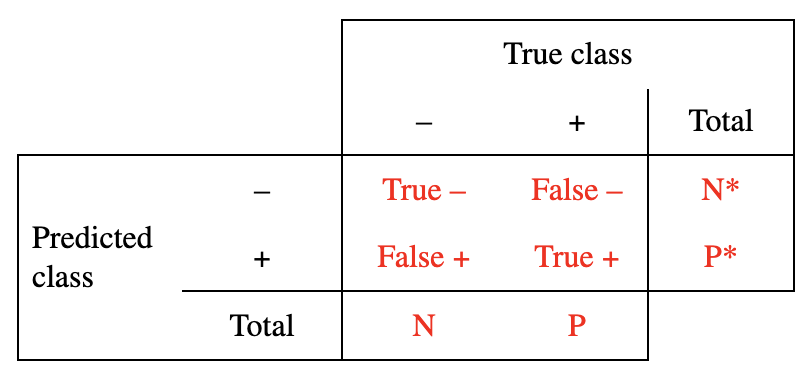
\includegraphics[width=3.33333in,height=\textheight]{images/confusionmatrix.png}

}

\end{figure}

The red text is where the numbers are filled in.
\end{column}

\begin{column}{0.4\textwidth}
\begin{itemize}
\item
  N and P are the number of actual negatives and positives respectively
  in the training data.
\item
  N* and P* are the number of predicted negative and positives in the
  training data.
\end{itemize}
\end{column}
\end{columns}
\end{frame}

\begin{frame}{Threshold}
\protect\hypertarget{threshold}{}
Recall that the Bayes classifier assigns observations to the class for
with the posterior probability is the greatest. Since probabilities sum
to 1, for a binary classifier this means that a test will come back
positive if:

\[
\operatorname{Pr}( \text{positive} \mid X=x) > 0.5
\]

That is, the binary classifier uses a threshold of 50\%. Depending on
the classification problem, one may want to specify a different
threshold level. For example:

\[
\text{positive if }\operatorname{Pr}( \text{positive} \mid X=x) > 0.2
\]
\end{frame}

\begin{frame}{ROC}
\protect\hypertarget{roc}{}
The ROC (receiver operator characteristics) curve is a method for
visualising the errors previously discusses for all possible thresholds.

\begin{columns}[T]
\begin{column}{0.5\textwidth}
\begin{figure}

{\centering 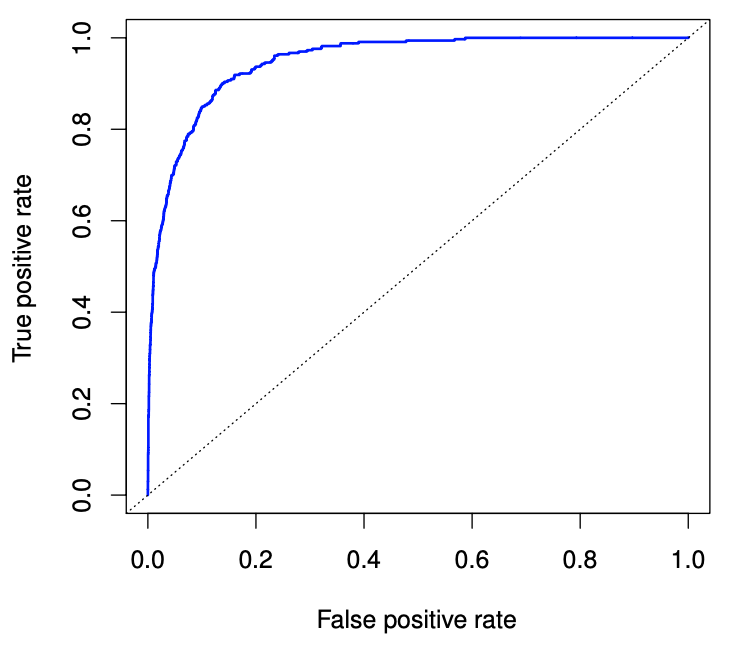
\includegraphics[width=2.38542in,height=\textheight]{images/ROC.png}

}

\end{figure}
\end{column}

\begin{column}{0.5\textwidth}
\begin{itemize}
\item
  Performance of a classifier is given by the area under the ROC curve,
  called the AUC.
\item
  The larger the AUC the better.
\item
  Ideal ROC curve is as close to the top left corner as possible.
\end{itemize}
\end{column}
\end{columns}
\end{frame}

\begin{frame}{Exercise: Linear Discriminant Analysis}
\protect\hypertarget{exercise-linear-discriminant-analysis}{}
Open the Classification Exercises R Markdown file.

\begin{itemize}
\item
  Go over the ``Linear Discriminant Analysis'' section together as a
  class.
\item
  5 minutes for students to complete the questions from ``Linear
  Discriminant Analysis''.
\item
  Questions should be completed at home if time does not allow.
\end{itemize}
\end{frame}

\begin{frame}{Quadratic Discriminant Analysis}
\protect\hypertarget{quadratic-discriminant-analysis}{}
The Quadratic discriminant analysis (QDA) classifier assumes that:

\begin{itemize}
\item
  observations are drawn from a class-specific Gaussian distribution
\item
  each class has its own covariance matrix (unlike LDA)
\end{itemize}

The QDA uses estimates for the class-specific means (\(\mu_k\)),
covariance matrices (\(\boldsymbol{\Sigma}_{k}\)), and prior probability
(\(\mu_k\)) to assign an observation \(x\) to the class for which

\[
\delta_{k}(x)=-\frac{1}{2}\left(x-\mu_{k}\right)^{T} \boldsymbol{\Sigma}_{k}^{-1}\left(x-\mu_{k}\right)-\frac{1}{2} \log \left|\boldsymbol{\Sigma}_{k}\right|+\log \pi_{k}
\] is the largest. Unlike the LDA, the function for \(\delta_{k}(x)\) is
quadratic which gives the QDA it's name.
\end{frame}

\begin{frame}{LDA vs QDA}
\protect\hypertarget{lda-vs-qda}{}
When to use the LDA versus the QDA:

\begin{itemize}
\item
  LDA is better than QDA when there are few training observations since
  it requires fewer parameters to be estimated.
\item
  QDA is best when there are many training observations or when the
  assumption of a common covariance matrix in the LDA is clearly wrong.
\end{itemize}
\end{frame}

\begin{frame}{Exercise: Quadratic Discriminant Analysis}
\protect\hypertarget{exercise-quadratic-discriminant-analysis}{}
Open the Classification Exercises R Markdown file.

\begin{itemize}
\item
  Go over the ``Quadratic Discriminant Analysis'' section together as a
  class.
\item
  5 minutes for students to complete the questions from ``Quadratic
  Discriminant Analysis''.
\item
  Questions should be completed at home if time does not allow.
\end{itemize}
\end{frame}

\begin{frame}{Naive Bayes}
\protect\hypertarget{naive-bayes}{}
The naive Bayes classifier assumes:
\textit{within each class, the $p$ predictors are independent}. This
allows us to disregard any association between the \(p\) predictors and
gives the form of \(f_k(x)\) as \[
f_{k}(x)=f_{k 1}\left(x_{1}\right) \times f_{k 2}\left(x_{2}\right) \times \cdots \times f_{k p}\left(x_{p}\right)
\] where \(f_{k j}\) is the density function of the \(j\)th predictor
for observations in the \(k\)th class.

To estimate \(f_{k j}\) using the training data there are several
options:

\begin{itemize}
\item
  For quantitative \(X_j\):

  \begin{itemize}
  \item
    assume that for each class, the \(j\)th predictor is drawn from a
    normal distribution, or
  \item
    estimate it as the fraction of the training observations in the
    \(k\)th class that belong to the same histogram bin as \(x_j\).
  \end{itemize}
\item
  For quantitative \(X_j\):

  \begin{itemize}
  \tightlist
  \item
    count the proportion of training observations for the \(j\)th
    predictor that belong to each class.
  \end{itemize}
\end{itemize}
\end{frame}

\begin{frame}{Exercise: Naive Bayes}
\protect\hypertarget{exercise-naive-bayes}{}
Open the Classification Exercises R Markdown file.

\begin{itemize}
\item
  Go over the ``Naive Bayes'' section together as a class.
\item
  5 minutes for students to complete the questions from ``Naive Bayes''.
\item
  Questions should be completed at home if time does not allow.
\end{itemize}
\end{frame}

\begin{frame}{\(K\)-Nearest Neighbours}
\protect\hypertarget{k-nearest-neighbours}{}
The \(K\)-nearest neighbors (KNN) classifier works very differently than
any of the previous classification methods. For a test observation
\(x_0\), it identifies \(K\) training data points that are closest to
\(x_0\) (represented by \(\mathcal{N}_0\)) and estimates the conditional
probability for class \(j\) as \[
\operatorname{Pr}\left(Y=j \mid X=x_{0}\right)=\frac{1}{K} \sum_{i \in \mathcal{N}_{0}} I\left(y_{i}=j\right)
\] where \(I(y_i = j)\) if an \textbf{indicator variable} that equals 1
is \(y_i = j\) and 0 otherwise. The KNN classifier classifies the test
observation \(x_0\) to the class for which the above probability is the
largest.
\end{frame}

\begin{frame}{\(K\)-Nearest Neighbours}
\protect\hypertarget{k-nearest-neighbours-1}{}
These figures illustrate the KNN approach with \(K=3\). To the left we
see the 3 closest points to x are 1 orange and 2 blue so this
observation will be classified as blue. The right figure shows the
decision boundaries where an observation will be classified as blue or
orange.

\begin{figure}

{\centering 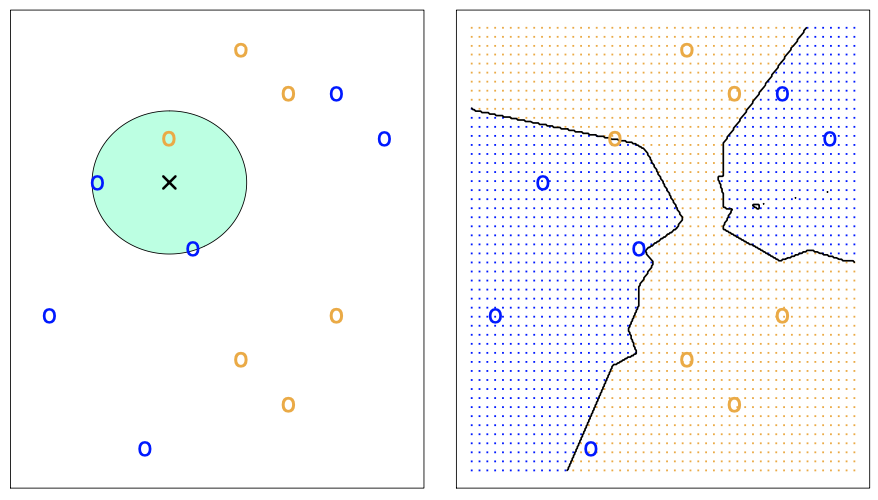
\includegraphics[width=3.125in,height=\textheight]{images/KNN1.png}

}

\end{figure}
\end{frame}

\begin{frame}{Exercise: K-Nearest Neighbours}
\protect\hypertarget{exercise-k-nearest-neighbours}{}
Open the Classification Exercises R Markdown file.

\begin{itemize}
\item
  Go over the ``K-Nearest Neighbours'' section together as a class.
\item
  5 minutes for students to complete the questions from ``K-Nearest
  Neighbours''.
\item
  Questions should be completed at home if time does not allow.
\end{itemize}
\end{frame}

\begin{frame}{How to choose the classification method}
\protect\hypertarget{how-to-choose-the-classification-method}{}
The choice of classification method depends on two things:

\begin{itemize}
\item
  the true distribution of the predictors in each of the \(K\) classes,
  and
\item
  the number of training observations (\(n\)) compared to to the number
  of predictors (\(p\)).
\end{itemize}
\end{frame}

\begin{frame}{References}
\protect\hypertarget{references}{}
Chapter 4 and section 2.2.3 of the ISLR2 book:

James, Gareth, et al.~An Introduction to Statistical Learning: with
Applications in R, 2nd ed., Springer, 2021.
\end{frame}



\end{document}
